\chapter{Background}
% First list what is going to be done in this chapter (outline)
In this section, we will review the relevant concepts and technologies that are necessary to understand the rest of the work. The topics are organized in two sections, Cyber Threat Intelligence Sharing and Dataspaces. The former will discuss the current state of the CTI sharing, its goals, and it challenges. The latter will analyse data spaces, its context and what it promises. Our goal is set the stage for our later discussions on how the data spaces could facilitate CTI sharing. 

\section{Cyber Threat Intelligence Sharing}
% In this section we will present the concept of \gls{cti} in more detail to understand why is it important, what are the 
% TODO: overview of the section
\subsection{Overview of Cyber Threat Intelligence}

\subsubsection{Intelligence}
We start with the term intelligence. 
Intelligence is often is associated with a state defense, an example intelligence organization is the Central Intelligence Agency (CIA). 
However, it could be relevant in the private sector as well. 
A relevant concept here is the Competitive Intelligence which is about gaining marketplace competitiveness through researching the market rivals. The intelligence definition that we will use throughout this thesis is the following:

\smallskip
The process and the product of the process of collecting, analysing and disseminating the information which is helpful in decision making.

To ensure the effectiveness, a systematic approach to intelligence is necessary. Therefore a lifecycle is often mentioned in the litereture to explain all the stages in the process. It consists of 6 stages that follow each other in circle, where each one builds on the previous one (Figure \ref{fig:cti-lifecycle}).

\begin{figure}[ht]
    \centering
    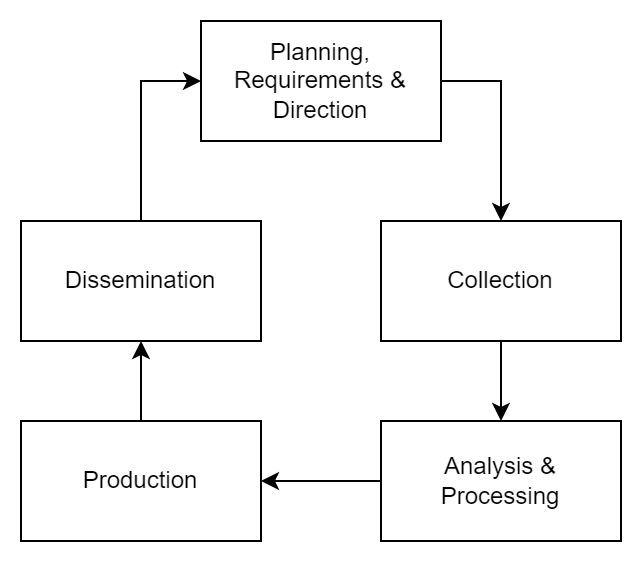
\includegraphics[width=0.5\textwidth]{diagrams/background/intelligence-cycle.png}
    \caption{The Intelligence Cycle \cite{lee_cyber_2023}}
    \label{fig:cti-lifecycle}
\end{figure}

\subsubsection{Cyber Threat Intelligence}
% Why CTI and why (already in motivation?)
By applying the provided definition of intelligence to the context of cyber security we could define Cyber threat intelligence (CTI) as follows:

\smallskip
The process of collecting, analyzing, and disseminating information about potential or current cyber threats. 

CTI is an important part of the security posture of any organization, because a constant study of cyber threats is necessary to mitigate and prevent cyber incidents.
It is due to the increase in the attack surface following the digitalization and emergence of new attack vectors developed by the threat actors, hence a constant evolution of the threat landscape.

\subsubsection{CTI Types and Goals}
CTI relies on collecting data from diverse sources, including security tools, threat feeds, honeypots, forums, social media platforms, and other relevant online and offline sources. It could be categorized into three different levels, each concerning different aspects of the threat landscape and different stakeholders. These are strategic, tactical, and technical CTI \cite{lee_cyber_2023}:

\paragraph{Strategic CTI -- Why?}
Strategic CTI expresses high level insights such as overall threat landscape, the motivations of threat actors, and the business or political impact of the threats. It mainly benefits executive management and other decision making departments by allowing data driven decision making to reduce the risks of cyber attacks.

\paragraph{Tactical CTI -- How?}
Tactical CTI is about "how" the threats can cause incidents. Examples are the tactics, techniques, and procedures (TTPs) used by threat actors, vulnerabilities in the organization's security infrastructure, and the strategies that were used to mitigate the impact of the breach. Security teams can achieve more efficiancy by not repeating the work already done leading to more agile cyber incident response.

\paragraph*{Technical CTI -- What?}
Technical CTI concerns with the indicators of compromise, meaning concrete technological signs about the attacker or an attack, such as malware hashes or malicious IP addresses. Another term for these products is the Indicator of Compromise (IoC), which refer to any technical observable showing an undergoing attack. Security teams and system administrators can feed IoCs to the firewalls and intrusion prevention systems (IPSs).

\subsection{CTI Sharing in Practice}
% TODO: outline

\subsubsection{The Role of Collaboration}
Organizations could improve their CTI capabilities through collaboration \cite{zibak_cyber_2019}. They can collaborate by sharing their findings with each other which we call CTI sharing. There are several benefits of sharing in the literature. \cite{zibak_cyber_2019} categorizes them into four categories: operational, organizational, economic, and policy related benefits. First, the operational benefits include reduce duplicate information handling and support breach detection and response. Second, organisational benefits such as improving overall security posture and situational awareness, combating skills gap, cross-checking different sources, and expanding professional networks. Third, economic benefits which are total cost savings, allowing governmental subsidies, reducing investment uncertainties. Lastly, policy related benefits such as reinforcing the connection with the government agencies.

\subsubsection{Collaboration Communities}
\label{subsubsec:collaboration-communities}
The current collaboration communities could be segregated into three different types, namely peer, commercial, and government \cite{connolly_trusted_2014}:

\paragraph{Peer Communities}
Peer communities are the most common type \cite{connolly_trusted_2014}. These collaboration happen in a community of participants with shared goals where they know and trust each other by means of meetings and so on. An example type of existing sharing communities are Information Sharing and Analysis Centers (ISACs), which are non-profit organizations that help organizations in a specific sector, usually a critical national infrastructure, e.g. electricity, water, gas, health care, finance, etc., to share CTI with each other. 

\subparagraph{EE-ISAC}
An example ISAC would be European Energy Information Sharing and Analysis Center (EE-ISAC) which has acquired over 30 members from utilities, academia, governmental and non-governmental organizations since its foundation in 2015. Members exchange cyber threat information through plenary meetings, working groups, and a dedicated platform (based on MISP). 
The information exchange is based on a trust achieved by confidentiality agreements and regular physical meetings with the same members. 
\cite{wallis_ee-isacpractical_2022}

Another type of peer communities are in the form of Open Source Intelligence (OSINT). There communities are accessible via internet and accessible via everyone, public CTI feeds, online forums, or social media accounts (e.g. Twitter) are common channels of OSINT.

\paragraph{Commercial Communities}
Commercial communities are the second type of collaboration communities. These are usually managed by a third party, and the participants pay a fee to access the shared information. The third party is responsible for the quality of the information and the trust between the participants. It also often annonimizes the information to protect the privacy of the participants. iDefense, Symantec, McAfee, Mandiant, Arbor Networks, and CrowdStrike are some examples of commercial communities.

\paragraph{Government Communities}
Finally, the communities managed by the government which form a public-private partnership (PPP) with either mandatory or voluntary participation are the third type. 

\subsubsection{CTI Channels and Automation}
\label{subsubsec:cti-channels}
There are various channels for CTI exchange. \cite{wagner_cyber_2019} mentions meetings, E-mails and phonecalls, shared databases, web portals or data feeds. Currently sharing CTI requires a lot of manual labor not only on the provider side, to prepare the information, but also on the consumer side to ingest the data by analyze the quality and relevance of the data and import it to local systems \cite{wagner_cyber_2019}. There means for automated sharing and consumption of CTI has emerged. It is not expected in the near future to drop the security analyst from the loop completely, but it tries to speed up the whole process \cite{wagner_cyber_2019}. To enable expressing CTI in a machine readable format, several protocols have been created  (Table \ref{tab:cti-protocols})

\begin{table}[ht]
    \label{tab:cti-protocols}
    \centering
    \begin{tabular}{|p{0.5\textwidth} p{0.5\textwidth}|}
    \hline
    \textbf{Title} & \textbf{Description} \\
    \hline
    \hline
    Structured Threat Information eXpression (STIX) \cite{stix_documentation_2024} & Structured language for CTI sharing (human and machine readable in JSON) \\
    \hline
    Trusted Automated eXchange of Indicator Information (TAXII) \cite{stix_documentation_2024} & Language to share CTI (open transport mechanism with native support for HTTP and HTTPS) \\
    \hline
    Malware Attribution Enumeration and Characterization (MAEC) \cite{maec_project_documentation_2024} & A standardized langauge for sharing structured information about malware (human and machine readable in XML) \\
    \hline
    Incident Object Description Exchange Format (IODEF) \cite{kampanakis_incident_2017} & Framework for sharing computer security incidents in XML \\
    \hline
    Vocabulary for Event Recoding and Incident Sharing (VERIS) \cite{veris_framework} & Language to describe structured security events \\
    \hline
    \end{tabular}
    \caption{CTI Protocols \cite{wagner_cyber_2019}}
\end{table}

\subsubsection{Sharing Models and Platforms}

As shown in \ref{fig:sharing-models}, there are three types of sharing. First, peer to peer, which is a direct exchange, second, peer to repository which allow for subscription to published events, and third, a hybrid model that incorporates the mentioned models.

\begin{figure}[ht]
    \centering
    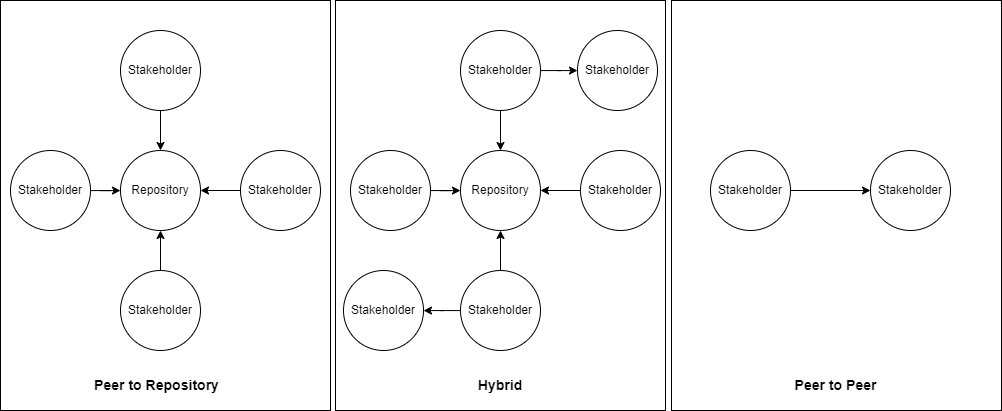
\includegraphics[width=\textwidth]{diagrams/background/sharing_models.png}
    \caption{Information Sharing Models \cite{wagner_cyber_2019}}
    \label{fig:sharing-models}
\end{figure}

\subsubsection{Threat Intelligence Platfrorms (TIPs)}
Another approach to accomplish a CTI repository is through Threat Intelligence Platforms (TIPs). Although there is no clear defintion of the scope of these platforms \cite{sauerwein_threat_2017}, they typically allow sharing CTI between users as well as collection of CTI from various sources (e.g. OSINT, 3rd party intelligence). However, some only focus on IOCs to be shared, allowing integration to interanal security systems such as Firewall, Intrusion Prevention Systems (IPSs), and Security Information and Event Management (SIEM) for an automated response \ref{fig:tip}. A list of available TIPs are in mentioned in table \ref{tab:tips}. \cite{sauerwein_threat_2017} provides a good survey of these platforms.

\begin{figure}[ht]
    \centering
    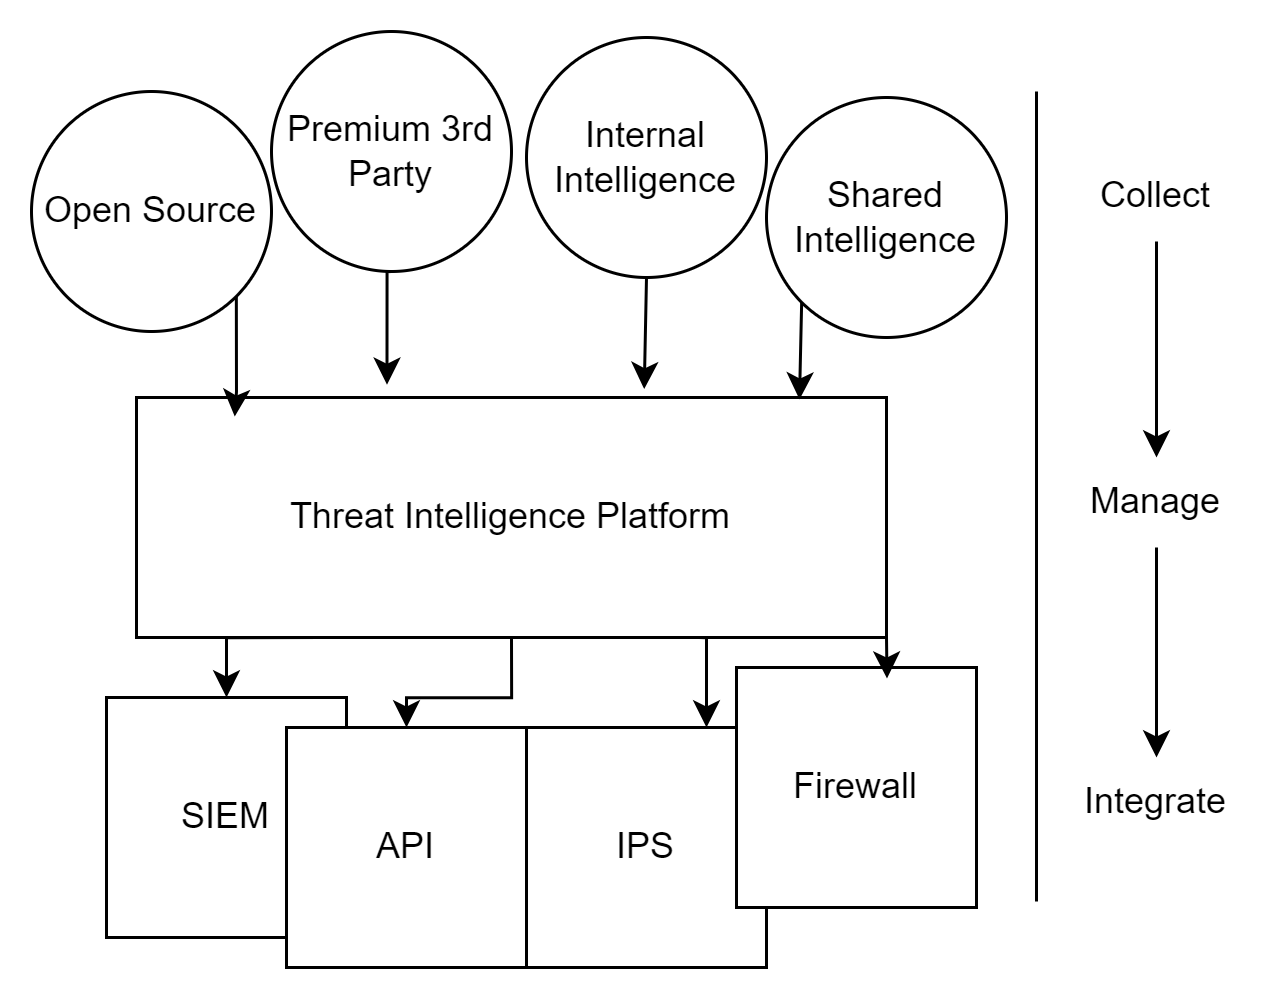
\includegraphics[width=\textwidth]{diagrams/background/threat-intelligence-platform.png}
    \caption{Threat Intelligence Platform (TIP) \cite{anomali_tip_2024}}
    \label{fig:tip}
\end{figure}

\begin{table}[ht]
    \centering
    \label{tab:tips}
    \begin{minipage}{\textwidth}
        \begin{tabular}{l c c}
            \textbf{TIP} & \textbf{Paid} & \textbf{Open Source} \\
            \hline
            Malware Information Sharing Platform (MISP) \footnote{https://www.misp-project.org} & & \checkmark \\
            Anomali ThreatStream \footnote{https://www.anomali.com/products/threatstream} & \checkmark & \\
            ThreatConnect \footnote{https://threatconnect.com} & \checkmark & \\
            ThreatQ \footnote{https://www.threatq.com/} & \checkmark & \\
            EclecticIQ Platform \footnote{https://www.eclecticiq.com/} & \checkmark & \\
            OpenCTI \footnote{https://filigran.io/solutions/products/opencti-threat-intelligence/} & \checkmark & \checkmark \\
            IBM X-Force Exchange \footnote{https://exchange.xforce.ibmcloud.com/} & & \\
            AlienVault Open Threat Exchange (OTX) \footnote{https://otx.alienvault.com/} & & \\
            CrowdStrike \footnote{https://www.crowdstrike.com/} & \checkmark & \\
            \hline
        \end{tabular}
    \end{minipage}
    \caption{Threat Intelligence Platforms}
\end{table}

\subsubsection{Regulations and Recommendations}
\label{subsubsec:regulations}
The landscape of Cyber Threat Intelligence (CTI) sharing is heavily influenced by a complex web of regulations and recommendations. Two important regulations are General Data Protection Regulation (GDPR) and The Network and Information Systems (NIS) Directive. 

\paragraph{GDPR} aims to protect the personal data and privacy of individuals within the EU and addresses the transfer of personal data outside the EU. GDPR is highly relevant in the context of CTI due to the potential inclusion of personal data in the threat intelligence information, such as IP addresses, email addresses, and other identifying information. 

\paragraph{NIS} directive, adopted in Europe in 2016, aims at improving the overall level of cybersecurity across the EU \cite{nis_directive}. It mandates the EU states to establish a national Computer Security Response Teams (CSIRTs) to monitor, detect, and respond to cyber incidents. These CSIRTs are required to collect information from private sector and share this with other national CSIRTs. It recommends the globally accepted standards and best practices for CTI sharing, such as the STIX/TAXII protocols. On December 2020, the revised directive NIS2 was proposed. NIS2, aims to improve the cooperation between the EU member states and the private sector, by increasing the scope of the directive to include more sectors, and by introducing new requirements for the incident reporting and information sharing.

Apart from the regulations, there are also recommendations from standardization bodies that try to harmonize the CTI sharing. Three of the most important standardization efforts are from European Union Agency for Cybersecurity (ENISA), International Organization for Standardization (ISO), and National Institute of Standards and Technology (NIST).

The first one is the ENISA's "Proactive Detection Of Network Security Incidents" which aims to enhance the capabilities of CERTs in detecting network security incidents by utilizing both external information sources and internal monitoring tools. This report provides guidelines and best practices to proactively identify and respond to potential cyber threats, thus improving the overall cybersecurity posture within the European Union.
The second one is the ISO's "Information technology -- Security techniques -- information security management for intersector and inter-organizational communications", which offers a standardized framework for managing and protecting sensitive information across different sectors and organizations. This standard ensures that information security measures are consistently applied, enabling secure and effective communication and collaboration between entities.
The third one is the NIST's "Guide to Cyber Threat Information Sharing" which provides guidelines and best practices for sharing cyber threat information among organizations. This guide aims to enhance situational awareness and improve the collective defense against cyber threats by facilitating timely and actionable information exchange. It outlines the processes, policies, and technical aspects of effective cyber threat information sharing to help organizations mitigate risks and respond to incidents more efficiently.

The aspects that are addressed in each one is summarized in table \ref*{tab:standardization}. 

\begin{table}[ht]
    \centering
    \begin{tabular}{ | l | c c c | }
    \hline
    \textbf{Aspect} & \textbf{ENISA} & \textbf{ISO} & \textbf{NIST} \\ \hline
    Protection of shared information & \checkmark & \checkmark & \\
    Cyber security risk management &  & \checkmark & \\
    Privacy preservation in information sharing & \checkmark &  & \\
    Data format, protocols and standards &  &  & \checkmark \\
    Data quality improvement & \checkmark &  & \\
    Incident handling process & \checkmark & \checkmark & \\ 
    \hline
    \end{tabular}
    \caption{Aspects addressed by the different standardization efforts \cite{skopik_survey_2016}.}
    \label{tab:standardization}
\end{table}

\subsection{Challenges of CTI Sharing}
Despite the benefits of CTI sharing, there are several challenges that hinder the effective sharing of cyber threat intelligence. \cite{johnson_guide_2016} lists the following general challenges: Establishing Trust, Achieving Interoperability and Automation, Safeguarding Sensitive Information, protecting classified information, enabaling infromation consumption and publication. \cite{johnson_guide_2016} also mentions some challenges that are specific to the consumer side: infrustracture for accessing external information, evaluation of the quality of the information. These challenges are summarized in table \ref{table:barriers}.

\begin{table}[ht]
    \centering
    \begin{tabular}{| m{6cm} | m{3cm} | m{3cm} |}
    \hline
    \textbf{Name} & \textbf{Involved Actor} & \textbf{Category} \\
    \hline
    Achieving Interoperability and Automation & Both & Operational \\
    \hline
    Evaluating the Quality of Received Information & Consumer & Operational \\
    \hline
    Safeguarding Sensitive Information (PII, Organization Secrets, Classified Information) & Both & Regulatory \& Operational \\
    \hline
    Establishing Trust & Both & Organizational \\
    \hline
    Free Riding Effect & Both & Economical \\
    \hline
    Risk of Reputation Loss & Provider & Economical \\
    \hline
    Enabling Information Consumption and Publication (Infrastructure for automatic sharing of indicators) & Both & Technical \\
    \hline
    Accessing External Information (Infrastructure) & Consumer & Technical \\
    \hline
    \end{tabular}
    \caption{Barriers in Cyber Threat Information Sharing. Adopted from various sources \cite{johnson_guide_2016}, \cite{zibak_cyber_2019}.}
    \label{table:barriers}
\end{table}

\subsection{Related Works}
There are several works that try to address the challenges of CTI sharing. 

\subsubsection{Leveraging Blockchain Technology}
\cite{el-kosairy_survey_2023} provides a survey of existing literature on the use of blockchain technology in CTI sharing. They found that blockchain technology is promising in addressing the challenges of CTI sharing, such as privacy of participants by anonymous identity and at the same time ensuring quality of data and incentivizing the participants to share data due to blockchain based reward systems. However, they also mention that most works are still in the proof of concept phase and the implementation in real world scenarios such as specific industry sectors is not done yet. A notable example is the work of \cite{homan_new_2019} which uses Hyperledge Fabric as a backbone and its channel capabilities to share CTI with specific partners utilizing smart contracts to enforce the traffic light protocol (TLP). In another work, Pahleven et al. \cite{pahlevan_secure_2021} extend the technological capacity of TAXII using Distributed Ledger Technologies (DLT) to enable data non-repudiation and a publish-subscribe middleware to enable real-time sharing.
\subsubsection{Open Source CTI} Jesus et al. \cite{jesus_sharing_2023} investigated the state of the art of the open source CTI and found the barriers that have prevented the formation of any widely used open source CTI platform. 
The barriers mentioned are 1) Legal and regulatory (e.g. GDPR or intellectual property) 2) Interoperability (e.g. different formats) 3) Usefulness and return 4) Market factors (e.g. losing reputation, free-riding) 5) Trust in peers and adversarial usage 6) Confidentiality risks. After studying these barriers, as well as some technical gaps, they present a confidentiality and privacy analysis of sharing a large sample data set of CTI, to make the claim that it is possible to manage risks of sharing using simple techniques like sanitization. Finally, they propose a set of requirements and a reference architecture for an open source threat intelligence platform. 
\subsubsection{Encryption Based CTI Sharing} De Fuentes et al. \cite{de_fuentes_pracis_2017} presents a scheme called PRACIS to guarantee privacy in cybersecurity information sharing (CIS) networks. They leverage format-preserving and homomorphic encryption primitives to share STIX formatted incident data. They approach allow secure aggregation and forwarding of data in a publish-subscribe architecture. They present a prototype implementation and show that the costs incurred by their approach are easily affordable in real-world scenarios.
\subsubsection{Incidents Information Sharing Platform (I2SP)} 
As part of the Phoneix project \cite{phoenix}, Incidents Information Sharing Platform (I2SP), tries to secure European Electrical Power and Energy Systems (EPES) adhering to the NIS directive \cite{skias_pan-european_2021}. It uses the STIX/TAXII protocols to share CTI among the EPES stakeholders, incorporates advanced machine learning and federated learning processes to detect and mitigate coordinated attacks in the EPES. It is inspired by MeliCERTes \cite{noauthor_melicertescsp_2024} which is part of the European Strategy for Cyber Security.  MeliCERTes is a network for establishing confidence and trust among the national Computer Security Incident Response Teams (CSIRTs) of the Member States and for promoting swift and effective operational cooperation. Member States CSIRTs participate on an equal footing in the MeliCERTes Core Service Platform (CSP) within verified Trust Circles for sharing and collaborating on computer security incidents. \cite{noauthor_melicertescsp_2024}
\subsubsection{C3ISP} Chadwick et. al. \cite{chadwick_cloud-edge_2020} provide a   cloud-edge based data sharing infrastructure, a trust model and a deployment model to satisfy the requirements of four real-world sharing scenario. Their solution allows the data provider the specify the trust level and the desired sanitization approach. They validated their approach in four pilot projects.
\subsubsection{Miscellaneous}
\cite{repetto_adaptive_2023} presents an overarching security scheme and architecture to improve the security of service chains with a intelligence centered approach towards proactive defense and and autonomous response. It was the only work I found that mentions the use of Dataspaces in the context of CTI sharing, altough not delving in details. \cite{coppolino_building_2023} presents a framework for securing smart grids based on FIWARE platform by creating a digital twin complying with Common Information Model. It uses a SIEM system for security monitoring.
Paice and McKeown \cite{paice_practical_2023} validate the utilization of MISP in the UK energy sector by testing different sharing models implemented by MISP in a simulated environment. 
\subsubsection{Summary}
We can see that the CTI sharing is a hot topic in the cybersecurity community. Especially following the NIS directive and the lack of adequate technical framework to support it, the research in this area has increased. There are several works that try to address the challenges such as privacy and automation, each leveragin a different set of tools. Despite the suitablitity of Dataspaces for CTI sharing, we weren't able to identify any work that delves into the challenges of Dataspaces for CTI sharing. Furthermore, we couldn't find any work that addresses the requirements of data sovereignty and usage control directly in the context of CTI sharing. A comparison of the aspects and the goals of some of the related works is summarized in table \ref{tab:related-works}.

\begin{table}[ht]
    \centering
    \label{tab:related-works}
    \begin{tabular}{l c c c c c c}
        \textbf{Aspect} & \textbf{\cite{de_fuentes_pracis_2017}} & \textbf{\cite{homan_new_2019}} & \textbf{\cite{skias_pan-european_2021}} & \textbf{\cite{chadwick_cloud-edge_2020}} & \textbf{This Work} \\
        \hline
        Data Sanitization & \checkmark & \checkmark & \checkmark & \checkmark & \checkmark \\
        Sharing Policies & & & \checkmark & \checkmark & \checkmark \\
        Trust Modelling & & \checkmark & & \checkmark & \checkmark \\
        Energy Sector Application & & & \checkmark & & \checkmark \\
        Usage Control & & & & & \checkmark \\
        \hline
    \end{tabular}
    \caption{Aspects addressed in related works on CTI sharing}
\end{table}


\subsection{Conclusion}
Cyber Threat Intelligence (CTI) is a young field that is rapidly evolving. In this section, we have discussed this concept and its importance in the context of cybersecurity. We have also discussed the different types of it, the benefits of collaborative CTI sharing, some regulations and recommendations that influence the CTI sharing landscape, the current state of CTI sharing, the protocols that are used for CTI sharing, the sharing models and platforms that are used for CTI sharing, the challenges that hinder the effective sharing of cyber threat intelligence. In the next section, we will discuss the concept of dataspaces and how they can facilitate CTI sharing.

\section{International Data Spaces (IDS)}
% TODO: Introduction
\subsection{History of Dataspaces}
The term dataspaces term was first coined by Franklin et al. \cite{franklin_databases_2005} to describe a new abstraction in data management to solve the data integration problem that follows: An organization has interrelated data in diverse origins, encompassing databases, files with various formats, and web services. The task is to query or update the data.
Franklin et al. proposed a DataSpace Suppport Platform (DSSP) that helps developers by providing a single query language based on a unified view of the data sources. This implies a pay-as-you-go approach where physically moving and transforming the data is done only by demand. The same concept was applied for the use case of inter-organisational data exchange and integration in newer contexts. In this context, the term dataspace refers to the platform consisted of data sources in different organizations to do data exchange defined by a set of standards and protocols to enable interoperability. \cite{reiberg_what_2022}

\subsection{Goals of Dataspaces}
Apart from data sharing and integration, dataspaces can fulfill other requirements.
A crucial requirement, that makes dataspaces interesting, is the sovereignty of data. dataspaces can fulfill data sovereignty by keeping the data in the owner's side, and only sharing the metadata publicly.
Another requirement is governance of the dataspace. In order to facilitate the cooperation of different participants, a set of policies, rules and protocols should exist. To define them, a governance body is commonly expected to exist \cite{reiberg_what_2022}.
dataspaces should be open, meaning anyone complying with the policies should be able to join, which encourages a fair and non-monopolistic market. This entails an easy access, which means, anyone should be able to connect with a limited effort.
dataspaces are usually designed to be decentralized and federated, meaning, there is no entity having direct control over all data exchanges. Different participants can interact with each other directly. This emphasizes the role of interoperability. This is only possible when certain open standards are established. Consequently, dataspaces complying to the same standards can be embedded inside each other enabling cross-data-space exchange \cite{reiberg_what_2022}.

\noindent\fbox{%
    \parbox{0.95\textwidth}{%
    "Dataspaces are defined as: A federated, open infrastructure for sovereign data sharing, based on common policies, rules and standards." \cite{reiberg_what_2022}
    }%
}

\subsection{Data Sovereignty}
By the increase of the value of data in businesses and data becoming a commodity, protecting data using laws and regulations has become a necessity. Data sovereignty is concept that has arisen in this context. It refers to the right of the owner of the data to have control over their data. By default, if a party is processing data owned by another party, the processing party can technically do anything with the data. Data sovereignty tries to address this issue. One means of achieving data sovereignty is by using usage control. Usage control concerns with introducing and enforcing restrictions on what could (not) happen to the data. It is the generalized version of the traditional access control which only concerns with "who" rather than "how", "where", "why". The data owner defines the usage policies and the usage control mechanism enforces them \cite{eitel_usage_2021}. A technology that can enable data sovereignty is dataspaces.

\subsection{International Data Spaces (IDS)}
The International Dataspaces (IDS) is an initiative with the goal of creating a standard for a distributed software architecture for data exchange with sovereignty. It was launched in 2015 as a Fraunhofer research project funded by the German Federal Ministry for Education and Research \cite{otto_evolution_2022}. In 2016, the IDS Association (IDSA) was founded as a non-profit organization to continue the research. It resulted in definition of the IDS Reference Architecture Model (IDS RAM). The IDS RAM is the description of IDS components and their interactions without being technology specific \cite{otto_evolution_2022}. IDS RAM allows anyone to implement the IDS compliant components using any technology. The IDSA also provides a reference implementation of different IDS components called IDS Testbed \footnote{https://internationaldataspaces.org/offers/reference-testbed/}. 

\subsubsection{IDS Reference Architecture Model (IDS RAM)}
IDS RAM defines the following components \cite{otto_ids_2019}:
Connector, Identity Provider, IDS Broker, Clearing House, IDS Apps, App Store, Vocabulary Provider \cite{pettenpohl_international_2022}.
% \begin{itemize}
%     \item Connector: The connector is the interface between the IDS ecosystem and the data source. It is responsible for the data exchange and the enforcement of the usage control policies as well as authentication.
%     \item Identity Provider: authentication service managing identity information
%     \item IDS Broker: Manages the metadata (description and usage policies)
%     \item Clearing House: Audits the data exchange and manages the payment
%     \item IDS Apps: Process the exchanged data. Deployed within Connector.
%     \item App Store: Provides IDS apps
%     \item Vocabulary Provider: Offers vocabularies to describe and annotate data
% \end{itemize}
Furthermore, it conceptualizes the following roles for the participants:
Data Owner, Data Provider, Data Consumer, Data User, App Provider
\cite{pettenpohl_international_2022}.
% \begin{itemize}
%     \item Data Owner: Controls the data and defines usage policies and payment model.
%     \item Data Provider: Provides the data to the IDS ecosystem with respect to the policies defined by the data owner.
%     \item Data Consumer: Same as data provider but consumes the data.
%     \item Data User: Same as data owner but uses the data.
%     \item App Provider
%     \item ...
% \end{itemize}
% Usage Control:
Also, it defines the standards and procedures to ensure data sovereignty. It uses usage control to enforce the usage policies defined by the data owner. It uses the following components to do so: Usage Control Policy Management Point (UC PMP), Usage Control Policy Decision Point (UC PDP), Usage Control Policy Enforcement Point (UC PEP) \cite{otto_evolution_2022}.
The policies are defined in a machine-readable format which is an extension of the Open Digital Rights Language (ODRL) \cite{eitel_usage_2021}. These policies should be mapped to a specific policy language supported by the tool that enforces them. IDSA RAM mentions the following policy enforcement tools: MYDATA \footnote{https://www.dataspaces.fraunhofer.de/en/software/usage-control/mydata.html}, LUCON \footnote{https://www.dataspaces.fraunhofer.de/en/software/usage-control/lucon.html}, D° \footnote{https://www.dataspaces.fraunhofer.de/en/software/usage-control/d.html}. 
% Certification:
% TODO: Add more details about the certification process

\subsection{Related Initiatives}
\paragraph{Gaia-X}

Gaia-X is an initiative, launched in 2019, that aims to foster creation of an infrastructure that allows for free and easy exchange of data and services between organizations and evade the vendor lock-in imposed by current proprietary cloud and service providers. To do so, regulations and technical specifications that are based on European values, applicable to any existing cloud and edge technology stack are going to be defined. The goal is to bring transparency, controllability, portability and interoperability across data and services. By facilitating data collection and sharing between organizations, a vibrant data ecosystem across Europe and beyond could evolve. Gaia-X Association deliverables include federation services, common policy rules and an architecture of standards. Federation services can be utilized by the ecosystem participants to achieve a global interoperability, compliance and effortless set up. This includes, “Identity and Trust”, “Federated Catalog” and “Data Exchange services”. \cite{otto_role_2022}
% AISBL: Gaia-X Association
% Nodes, Services (Any cloud service), Service Instances (A service running on a node) and Data Assets (a data set on a node)
% Participants: Organizations and individuals that are part of the Gaia-X ecosystem
% Clearing House: Middle man in the exchange checking for compliance

% \paragraph{Big Data Value Association (BDVA)}


\paragraph{Comparison of IDS and Gaia-X}

% Mapping of Gaia-X to IDS
    % Federated Catalog ~ IDS Broker + Vocabulary Provider + Information Model
    % Identity and Trust ~ IDS Identity Provider + Dynamic Attribute Provisioning Service (DAPS)
    % Gaia X Sovereign Data Exchange ~ IDS Usage Control and Clearing House
    % Gaia X Node ~ IDS Connector

%  Why choose IDSA? 
    % Maturity
    % Open source Reference Implementation
    % Big picture cloud vs. data exchange

% TODO: 
    % IDSA: usage control
    % Gaia-X: Data at rest

In comparison to IDSA, Gaia-X is less mature and still in the development phase whereas IDSA is used in the industry\cite{otto_prof_dr_boris_gaia-x_2021}.
It focuses on cloud infrastructures and businesses operating within EU, in contrast to IDSA which is more on the technicalities of the sovereign data exchange\cite{otto_prof_dr_boris_gaia-x_2021}.
Finally, Gaia-X can use IDSA in the data exchange layer \cite{otto_prof_dr_boris_gaia-x_2021}. 

\paragraph{Other Data Spaces}
Other data management researches based on dataspaces include "Trusted Integrated Knowledge Dataspace For Sensitive Healthcare Data Sharing" (TIKD)  \cite{hernandez_tikd_2021}, which fulfills the following requirements: secure collaborative knowledge graph database of potentially personal data with fine grained access control and privacy-aware data interlinking.
Another example is Real-time Linked Dataspace (RLD) \cite{curry_real-time_2019} which is designed for the Smart Environments, supporting a pay-as-you-go data integration management system for real-time heterogeneous data sources that provides unified query interface based on linked data technologies.
However, these data spaces lack the data sovereignty and usage control features that are necessary for our use case.

\subsection{Application of IDS in Practice}
Dataspaces concept has been applied to many use cases in many sectors \cite{dataspace_radar}. IDSA publishes a list of all applications of Dataspaces in a report and tool called "Dataspaces Radar" \cite{dataspace_radar}. In the report for 2024, it mentions 145 entries in different sectors. It mentions the following sectors: Mobility, Automotive, Energy, Health, Manufacturing and many more.
Some notable examples are the following:

\paragraph{Advaneo} 
In the rapidly expanding fields of IoT, Industry 4.0, smart agriculture, and digital twins, where data generation is at an all-time high, IDS-based Data Spaces offer an ideal solution for connecting various domains and standards while ensuring full data sovereignty. The Advaneo Data Marketplace (DMP) \footnote{https://www.advaneo-datamarketplace.de/en/}, leveraging IDS architecture and future GAIA-X standards, serves as a collaboration platform that facilitates the formation of Data Spaces for data-driven applications.
It incorporates AI tools, data models, and applications, and provides access to millions of open data resources, supporting innovative data-driven projects. Key benefits for participants include access to diverse data sources, sovereign data sharing under IDS standards, on-the-fly data processing capabilities, opportunities for open innovation through datathons, and comprehensive access control within organizations. \cite{dataspace_radar}

\paragraph{Catena-X}
Catena-X \footnote{https://catena-x.net/de/} aims to establish a uniform standard for data exchange across the entire automotive value chain, utilizing the IDS standard, which is grounded in European principles such as data protection, security, and data sovereignty. This standard promotes equal opportunities through a federated design and ensures trust among participants. As a foundational infrastructure, the IDS standard allows Catena-X to evolve into a comprehensive ecosystem where automotive manufacturers, suppliers, dealer associations, equipment suppliers, and tech providers can participate on an equal footing. The benefits for participants include setting a crucial benchmark for tackling digital transformation challenges, boosting the automotive industry's competitiveness, enhancing operational efficiency through collaboration, and speeding up organizational processes by standardizing and facilitating access to data.

\paragraph{SCSN}
The \textbf{Smart Connected Supplier Network (SCSN)} \footnote{https://smart-connected.nl/en} is an initiative targeting the high-tech manufacturing sector, designed to improve supply chain transparency and interoperability. It aims to boost productivity by 20\%, primarily through reducing administrative burdens and enhancing collaboration among partners. Unlike conventional centralized platforms, SCSN is built on principles of \textit{digital and data sovereignty}, operating without centralized data control. SCSN employs a scalable network approach based on a four-corner model, which includes:
\begin{enumerate}
    \item A unified semantic language for exchanging a wide range of data, including orders, forecasts, technical product documentation (TPD), bills of materials (BoM), drawings, invoices, logistical information, catalogues, and measurement data.
    \item Seamless technical agreements between service providers, ensuring compliance with the \textit{International Data Spaces Association's} reference architecture. This system supports the premise of \textit{``Connecting Once - Communicate with Everyone"}.
\end{enumerate}

% \subsection{Energy Dataspaces}
% SKIPPED for now